% OT Security Monitor - projektrapport (redigerbar LaTeX-kalla)
% Kompilera: pdflatex OT_Security_Monitor_Report.tex (kor 2 ggr). Figurer i output/
%
\documentclass[11pt,a4paper]{article}
\usepackage[utf8]{inputenc}
\usepackage[T1]{fontenc}
\usepackage[protrusion=true,expansion=false]{microtype}
\usepackage{graphicx}
\usepackage[table,svgnames]{xcolor}
\usepackage[top=2cm,bottom=2cm,left=2.2cm,right=2.2cm]{geometry}
\usepackage{array}
\usepackage{tabularx}
\usepackage{enumitem}
\usepackage[colorlinks=true,linkcolor=NavyBlue,urlcolor=NavyBlue]{hyperref}
\usepackage{helvet}
\renewcommand{\familydefault}{\sfdefault}
\frenchspacing
\hyphenpenalty=10000 \exhyphenpenalty=10000 \tolerance=3000 \emergencystretch=3em
\setlength{\parindent}{0pt}\setlength{\parskip}{6pt}
\definecolor{th}{HTML}{0E5F7A}
\definecolor{rd}{HTML}{8A0018}
\newcommand{\secbar}[1]{\vspace{4pt}{\color{th}\large\bfseries #1}\par\vspace{-4pt}{\color{th}\rule{\linewidth}{1.2pt}}\par}
\newcommand{\secbarr}[1]{\vspace{4pt}{\color{rd}\large\bfseries #1}\par\vspace{-4pt}{\color{rd}\rule{\linewidth}{1.2pt}}\par}
\renewcommand{\arraystretch}{1.25}
\begin{document}

{\Huge\bfseries OT Security Monitor}\\[2pt]
{\large Fjärrvärme --- detektion av cyberangrepp i industriella miljöer (IT/OT)}\\[4pt]
{\color{gray}Demonstrationsprojekt för rollen Informationssäkerhetssamordnare vid ett energibolag (fjärrvärme) \\
Suraj Karki \quad\textbullet\quad MATLAB/Simulink \quad\textbullet\quad NIST CSF 2.0 / NIS2 / ISO 27001}

\vspace{6pt}
\noindent\fcolorbox{th}{th!8}{\parbox{\dimexpr\linewidth-2\fboxsep}{%
\textbf{Sammanfattning.} Systemet lär in normal fjärrvärmedrift från en ren baslinje och larmar
därefter på avvikelser: multivariata avvikelser (Mahalanobis-avstånd), brutna fysikaliska samband
(givarförfalskning) och förlorad telemetri (tillgänglighet). Fyra angreppsscenarier injiceras med
facit. \textbf{Resultat:} recall 78\,\%, precision 98\,\%, F1 0{,}87 över 7 dygns telemetri
(2016 sampel). Metodiken motsvarar strukturerad risk- och sårbarhetsanalys samt kontinuerlig
övervakning enligt NIST CSF 2.0 och kraven i NIS2/cybersäkerhetslagen. Ett kompletterande UEBA-lager bevakar dessutom konfidentialitet --- obehörig åtkomst till normala data (insiderhot, stulna inloggningsuppgifter, exfiltrering, privilegiemissbruk) --- med recall 100\,\% och precision 89\,\%.}}

\secbar{1. OT-telemetri och injicerade angrepp}
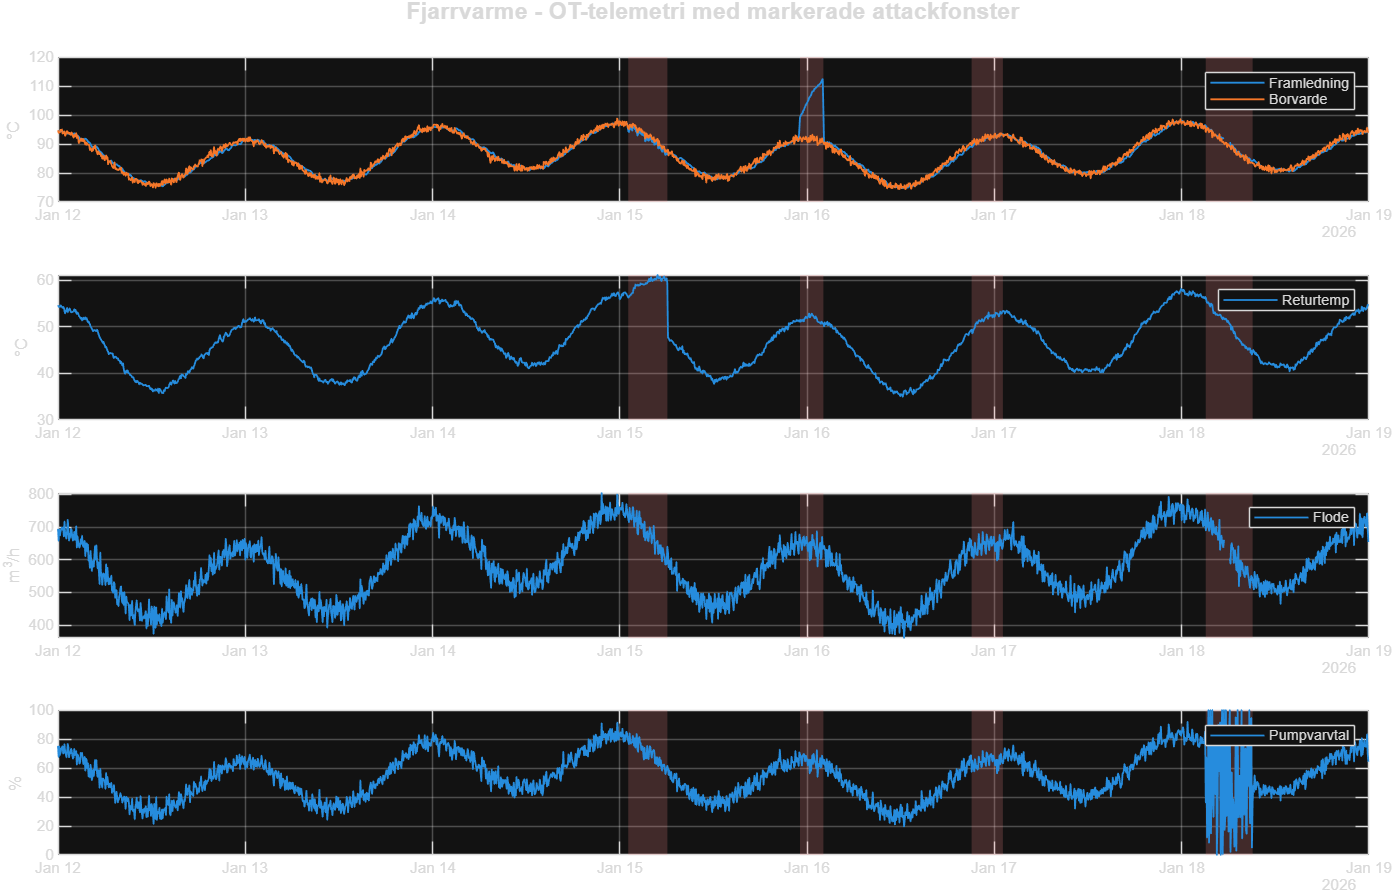
\includegraphics[width=\linewidth]{output/fig_telemetry.png}
{\color{gray}\small Fyra angreppsfönster (skuggade): sensor\-spoofing, command injection (överhettning),
replay och en ransomware-lik störning med fladdrande pump och förlorad telemetri.}

\secbar{2. Avvikelsedetektion}
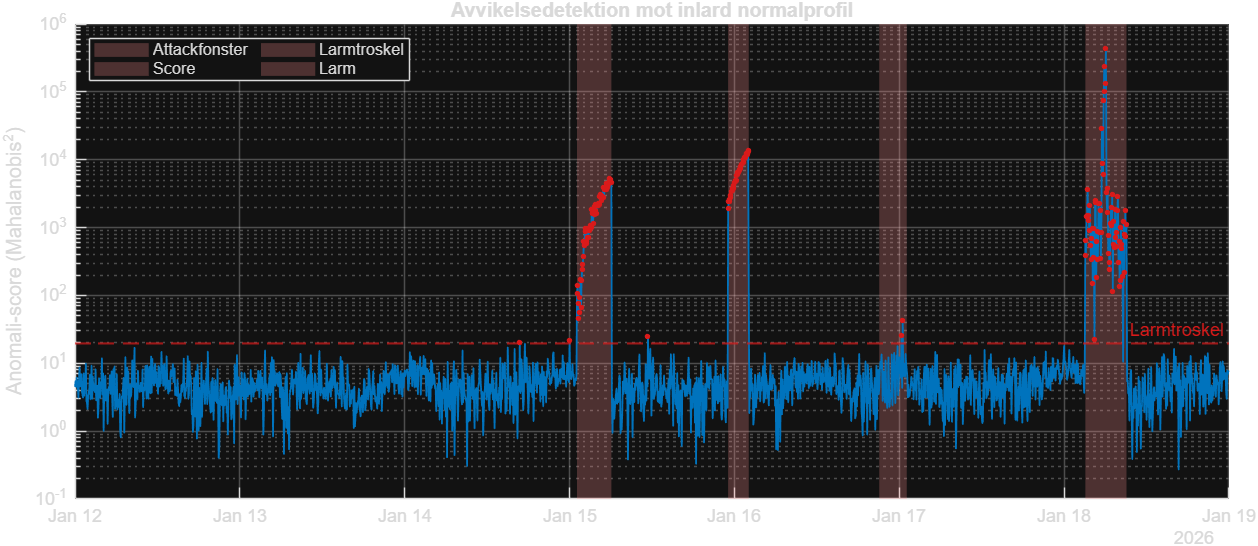
\includegraphics[width=\linewidth]{output/fig_detection.png}
{\color{gray}\small Anomali-score (Mahalanobis$^2$, log) mot inlärd normalprofil. Scoren ligger i
baslinjebandet vid normal drift och passerar larmtröskeln (röd) i varje angreppsfönster.
Detektionskvalitet: recall 78\,\%, precision 98\,\%, F1 0{,}87.}

\secbar{3. Incidenter}
\begin{tabularx}{\linewidth}{@{}c X l c c@{}}
\rowcolor{th}\color{white}\# & \color{white}\textbf{Scenario} & \color{white}\textbf{CSF} & \color{white}\textbf{Allvar} & \color{white}\textbf{Detekterad}\\
1 & Sensor spoofing (false data injection) & DE.AE / PR.DS & 4/5 & Ja\\
2 & Command injection (ändrat börvärde) & RS.MA / PR.AA & 5/5 & Ja\\
3 & Replay attack (uppspelning av historik) & DE.CM / PR.AA & 3/5 & Ja\\
4 & Ransomware-lik OT-störning & RC.RP / DE.CM & 5/5 & Ja\\
\end{tabularx}

\vspace{2pt}{\color{gray}\small NIS2 / cybersäkerhetslagen: tidig varning inom 24 h, incidentanmälan
inom 72 h och slutrapport inom en månad till MSB för väsentlig verksamhet.}

\secbar{4. Risk- och sårbarhetsanalys}
\begin{minipage}[t]{0.50\linewidth}
\vspace{0pt}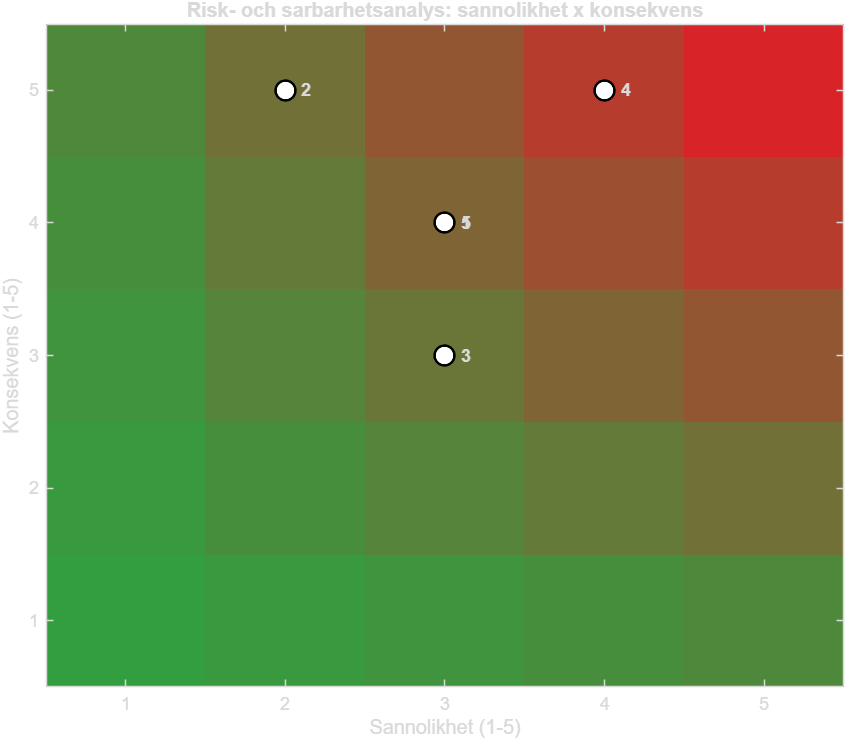
\includegraphics[width=\linewidth]{output/fig_risk.png}
\end{minipage}\hfill
\begin{minipage}[t]{0.46\linewidth}
\vspace{2pt}
\begin{tabularx}{\linewidth}{@{}X c c c@{}}
\rowcolor{th}\color{white}\textbf{Scenario} & \color{white}S & \color{white}K & \color{white}Risk\\
Sensor spoofing & 3 & 4 & 12\\
Command injection & 2 & 5 & 10\\
Replay attack & 3 & 3 & 9\\
Ransomware-störning & 4 & 5 & 20\\
Leverantörskedja & 3 & 4 & 12\\
\end{tabularx}
\par\vspace{4pt}{\color{gray}\small S = sannolikhet, K = konsekvens (1--5).}
\end{minipage}

\secbar{5. Koppling till NIST CSF 2.0}
\begin{tabularx}{\linewidth}{@{}l X@{}}
\rowcolor{th}\color{white}\textbf{Funktion} & \color{white}\textbf{Hur projektet adresserar den}\\
GOVERN & Riskaptit och prioritering via risk-/sårbarhetsanalys; leverantörsrisk (GV.SC).\\
IDENTIFY & Tillgångs- och dataflödeskartläggning (IT/OT), riskbedömning per scenario.\\
PROTECT & Segmentering IT/OT, MFA, härdning av styrsystem, immutabel backup.\\
DETECT & Kontinuerlig övervakning och avvikelsedetektion (denna monitor).\\
RESPOND & Incidentklassning, allvarsgrad och NIS2-rapporteringsfrister.\\
RECOVER & Åtgärdsförslag och kontinuitet vid tillgänglighetsstörning.\\
\end{tabularx}

\secbarr{6. Hotscenario: phishing $\rightarrow$ ransomware (MITRE ATT\&CK for ICS)}
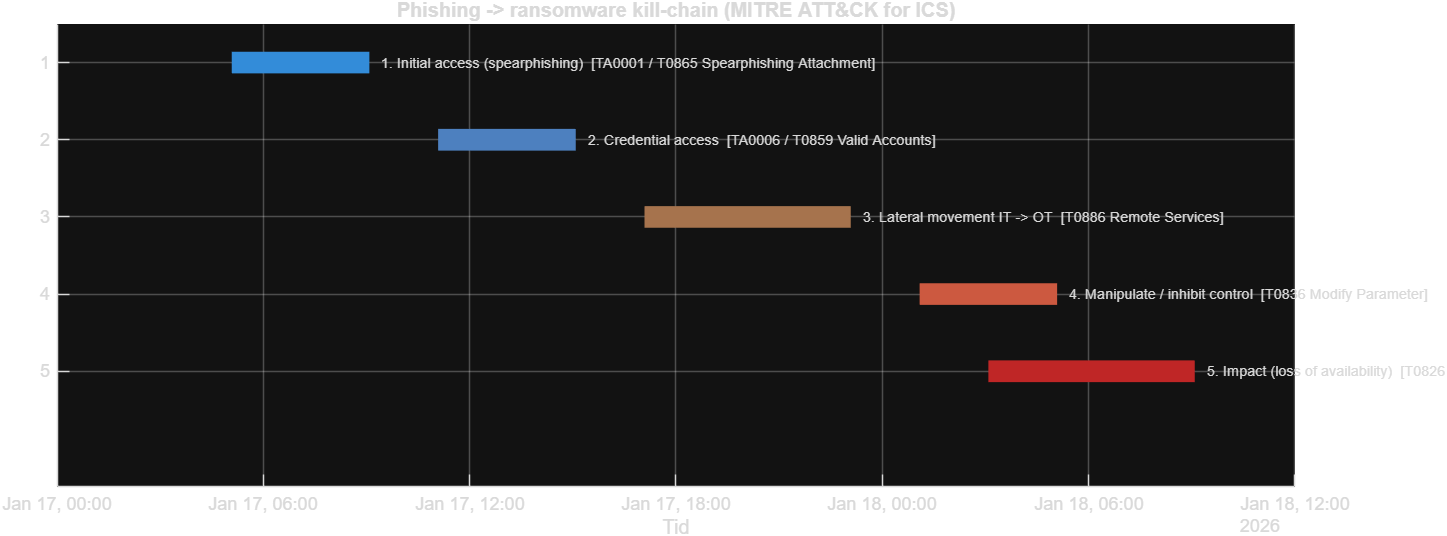
\includegraphics[width=\linewidth]{output/fig_killchain.png}
\begin{tabularx}{\linewidth}{@{}l l X@{}}
\rowcolor{rd}\color{white}\textbf{Steg} & \color{white}\textbf{ATT\&CK for ICS} & \color{white}\textbf{Försvarsåtgärd}\\
1. Initial access (spearphishing) & T0865 & Medvetenhet, e-postfiltrering, MFA\\
2. Credential access & T0859 & MFA, least privilege, kontoövervakning\\
3. Lateral movement IT$\rightarrow$OT & T0886 & Segmentering, zero-trust, jump-host\\
4. Manipulera/inhibera styrning & T0836 & Avvikelsedetektion, integritetsskydd\\
5. Impact (loss of availability) & T0826 / T0813 & Immutabel backup, IR-plan, NIS2\\
\end{tabularx}

\secbarr{7. IT-indikatorer (tidig förvarning)}
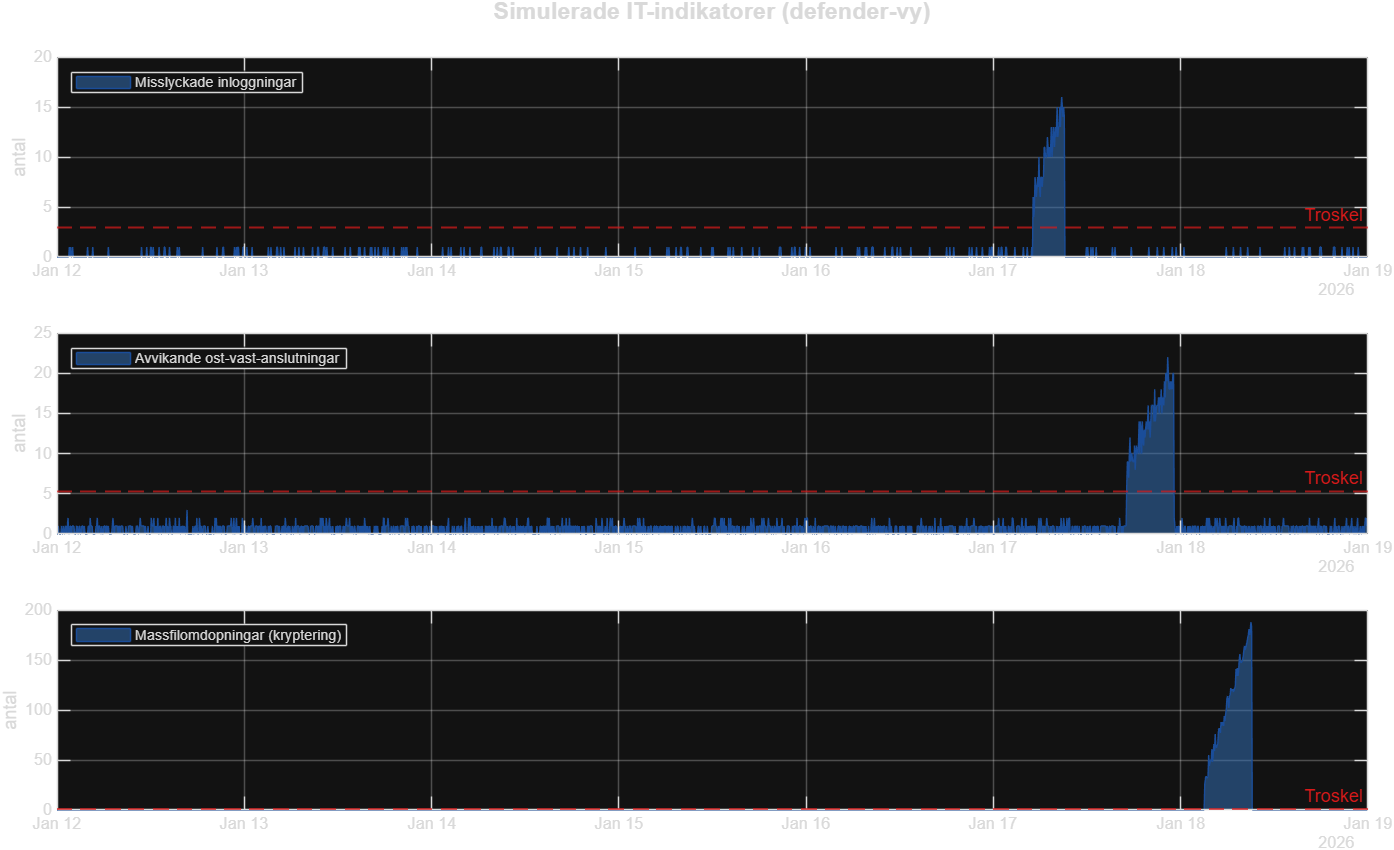
\includegraphics[width=\linewidth]{output/fig_indicators.png}
{\color{gray}\small Simulerade indikatorer eskalerar i tur och ordning --- misslyckade inloggningar
$\rightarrow$ avvikande öst-väst-trafik $\rightarrow$ massfilomdöpningar --- och passerar var sin
tröskel före OT-störningen, vilket ger tid för inneslutning och rapportering.}

\secbar{8. Rekommenderade åtgärder (NIST ransomware-profil)}
\begin{itemize}[leftmargin=1.4em,itemsep=1pt]
\item Offline/immutabla och testade säkerhetskopior av styrsystem och historik.
\item Segmentering och zero-trust mellan kontorsnät (IT) och produktionsnät (OT).
\item Phishing-resistent MFA och least privilege för åtkomst till styrsystem.
\item Kontinuerlig övervakning av nätverk, endpoints och givarsignaler.
\item Övad incidenthanterings- och återställningsplan med out-of-band-kommunikation.
\end{itemize}

\secbar{9. Live-vy: animerad uppspelning}
Funktionen \texttt{ot\_live} spelar upp telemetrin i realtid och larmar medan angreppen utvecklas,
med en rullande händelselogg. Bilden visar slutläget med samtliga larm markerade.
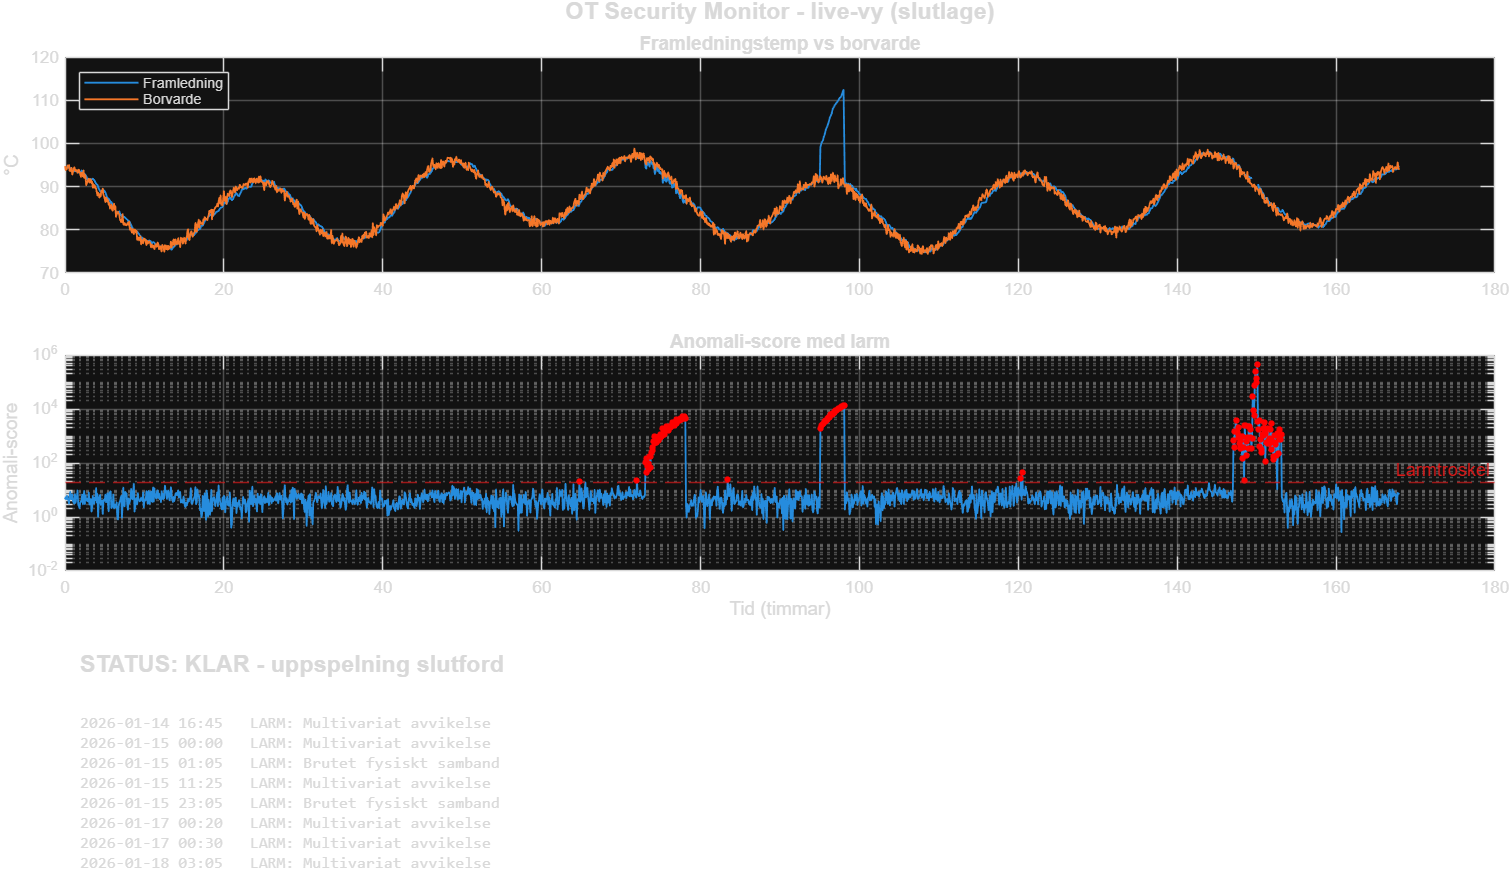
\includegraphics[width=\linewidth]{output/fig_live.png}

\secbar{10. Simulink-demo: strömmande dataflöde med funktionsblock}
Modellen \texttt{ot\_security\_demo} kör samma detektion som ett strömmande dataflöde: telemetrin
matas in, ett \textbf{AttackInjector}-block injicerar angrepp live utifrån klockan, och ett
\textbf{Detector}-block (MATLAB Function, med inlärd baslinje) beräknar anomali-score och ett
\textbf{LARM}-larm, kopplat till scope och loggning.
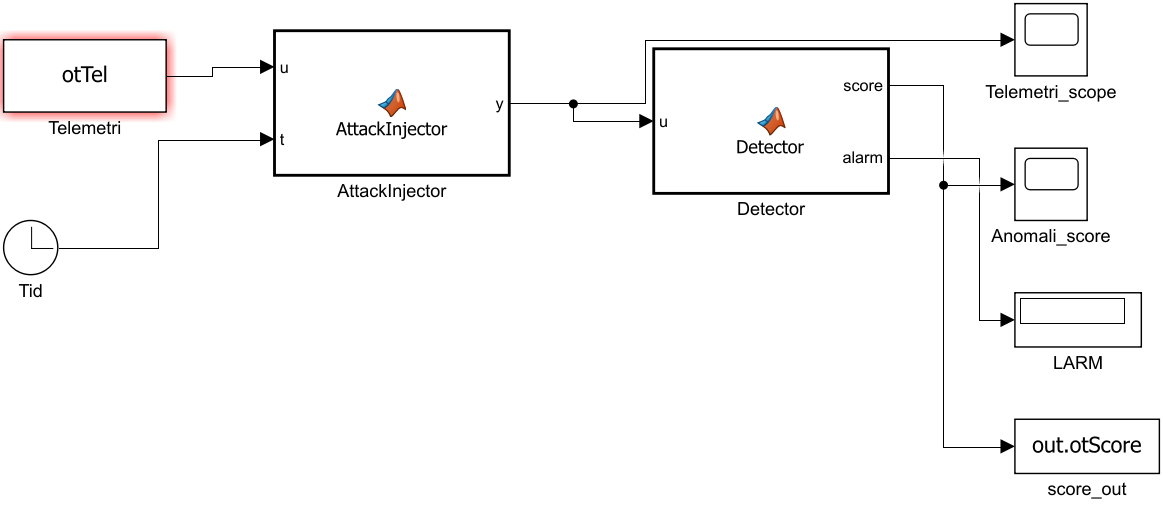
\includegraphics[width=\linewidth]{output/fig_simulink.png}

\secbar{11. Automatiserad incidentrapportering (NIS2 / GDPR / säkerhetsskydd)}
Modulen \texttt{ot\_autoreport} omvandlar varje detekterad incident till färdiga myndighets\-anmälningar.
Den klassar incidenten (typ, allvar, berörda regelverk), beräknar lagstadgade tidsfrister och fyller
automatiskt i anmälningsdokument: \textbf{NIS2}/cybersäkerhetslagen (tidig varning 24\,h, anmälan 72\,h,
slutrapport 1 månad till MSB), \textbf{GDPR} (anmälan till IMY inom 72\,h vid personuppgiftsincident) och
\textbf{säkerhetsskydd} (skyndsam anmälan). Utdata: ett incidentregister (CSV), ifyllda anmälningar per
incident och en översiktsdashboard.
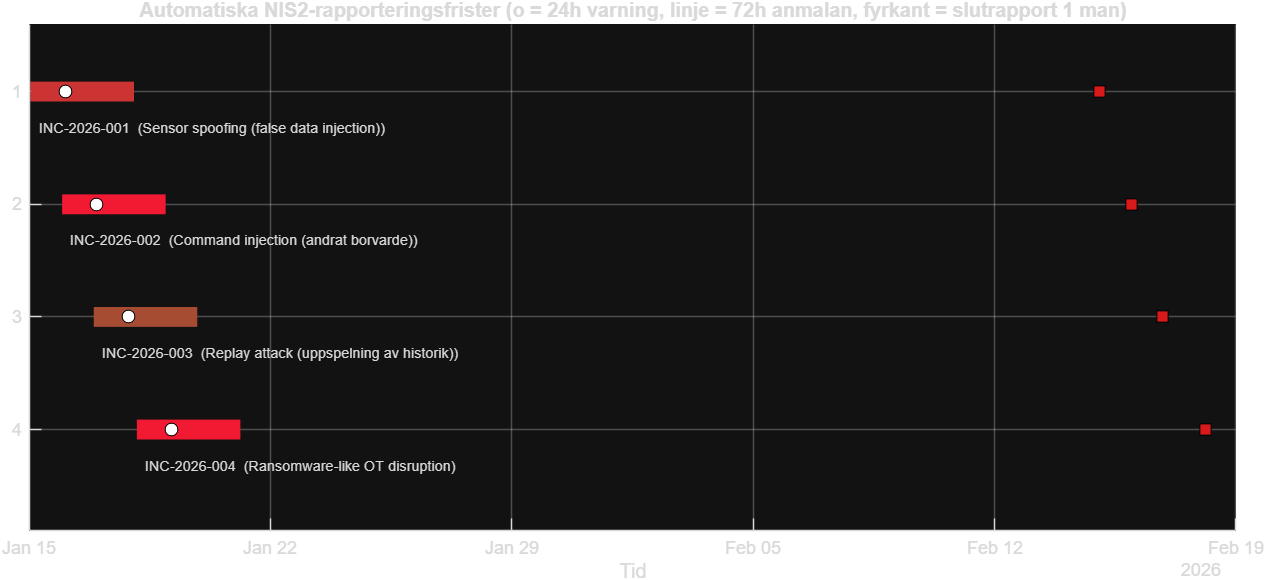
\includegraphics[width=\linewidth]{output/fig_deadlines.png}
\begin{tabularx}{\linewidth}{@{}l X c c c c@{}}
\rowcolor{th}\color{white}\textbf{ID} & \color{white}\textbf{Scenario} & \color{white}\textbf{Allvar} & \color{white}\textbf{NIS2 72h} & \color{white}\textbf{GDPR} & \color{white}\textbf{Säk.skydd}\\
INC-2026-001 & Sensor spoofing & 4/5 & 2026-01-18 01:05 & Nej & Nej\\
INC-2026-002 & Command injection & 5/5 & 2026-01-18 23:05 & Nej & Ja\\
INC-2026-003 & Replay attack & 3/5 & 2026-01-19 21:05 & Nej & Nej\\
INC-2026-004 & Ransomware-störning & 5/5 & 2026-01-21 03:05 & Ja & Ja\\
\end{tabularx}
{\color{gray}\small Registret skrivs även som CSV och varje rad länkar till en auto-ifylld anmälan.}

\secbar{12. Konfidentialitet: obehörig åtkomst och beteendeanalys (UEBA)}
Avsnitten ovan upptäcker när \emph{värdena} blir fel (integritet och tillgänglighet). Ett lika
allvarligt hot är \emph{normala värden i fel händer}: ett giltigt konto som läser, kopierar eller
exfiltrerar helt normal data. Då syns ingen avvikelse i processvärdena --- signalen finns i
\emph{vem} som gör \emph{vad}, \emph{när} och \emph{hur mycket}. Modulen \texttt{ot\_ueba} lär in
varje kontos normala beteende (arbetstider, datavolym, platser och resurser) från en ren baslinje och
poängsätter därefter varje åtkomst med Mahalanobis-avstånd, kompletterat med nyhetsstraff för okänd
plats eller resurs utanför rollen.

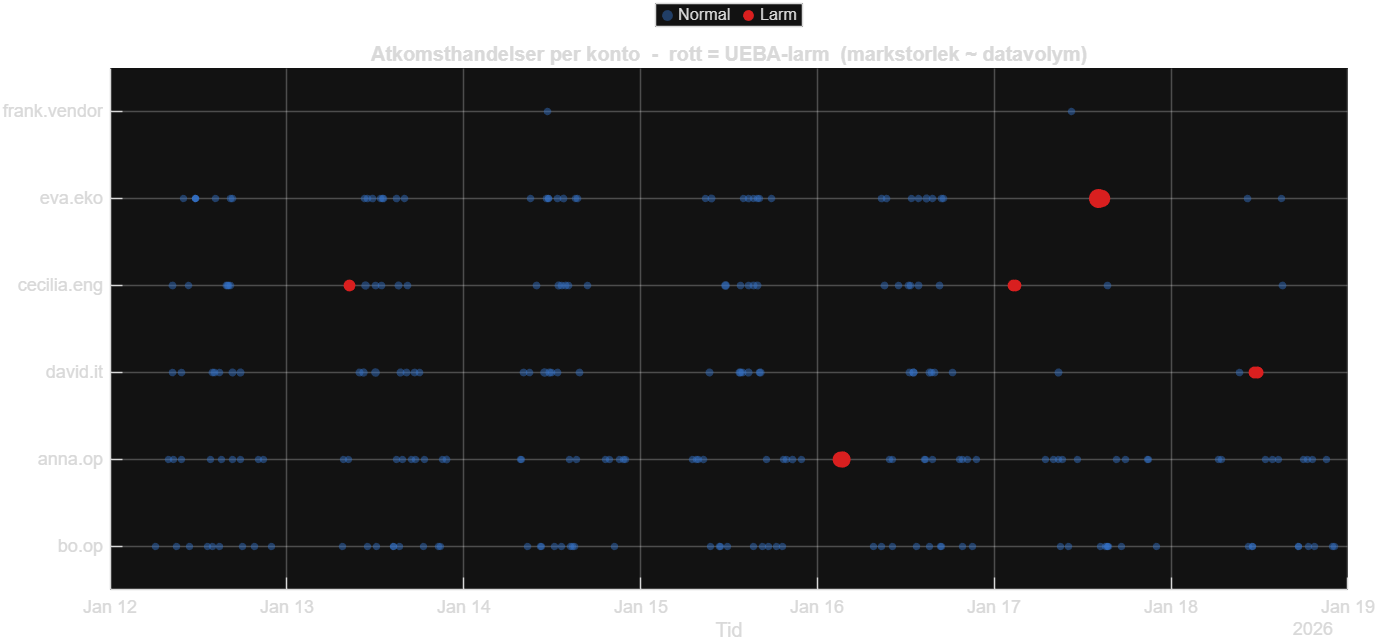
\includegraphics[width=\linewidth]{output/fig_access_timeline.png}
{\color{gray}\small Åtkomsthändelser per konto över sju dygn (markörstorlek $\sim$ datavolym). Röda
markörer är UEBA-larm --- varje injicerat fall är en giltig inloggning med helt normala OT-värden.}

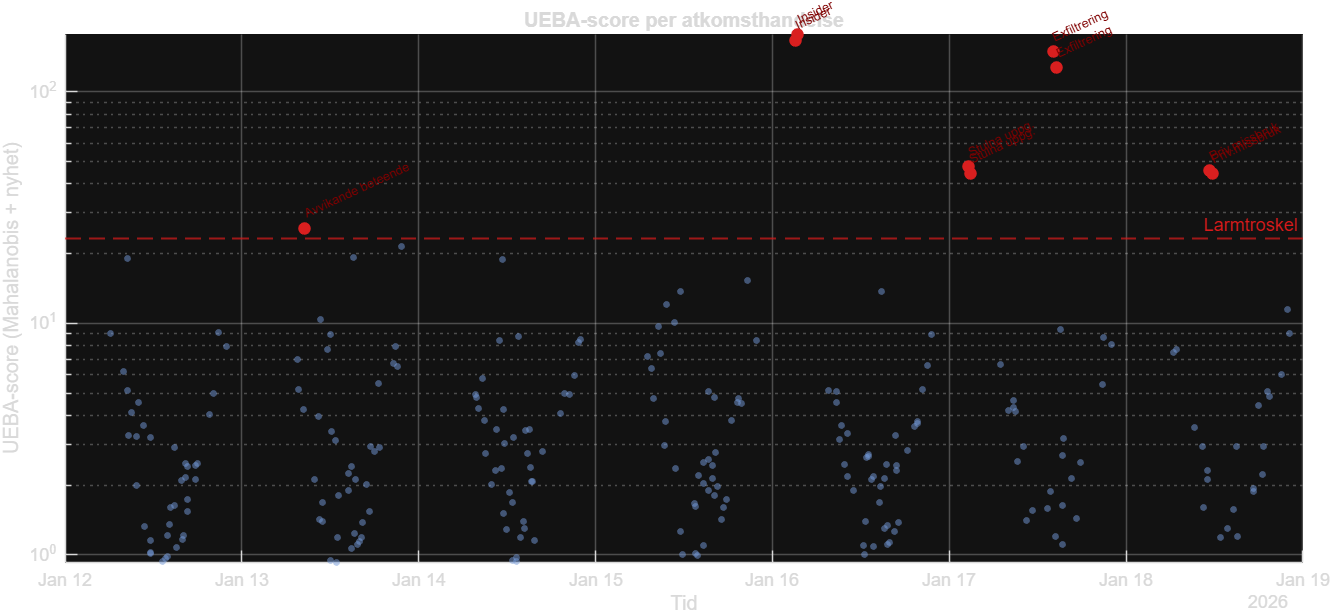
\includegraphics[width=\linewidth]{output/fig_ueba_scores.png}
{\color{gray}\small UEBA-score per åtkomst (Mahalanobis + nyhet, log-skala) mot inlärd baslinje. Normal
aktivitet ligger lågt; de fyra angreppstyperna passerar tydligt larmtröskeln och klassas automatiskt.}

\vspace{2pt}
\begin{tabularx}{\linewidth}{@{}l X l l@{}}
\rowcolor{th}\color{white}\textbf{Hot} & \color{white}\textbf{Signatur i åtkomstdata} & \color{white}\textbf{CSF} & \color{white}\textbf{Skydd}\\
Insidermissbruk & Egen resurs men avvikande tid och $\sim$40$\times$ datavolym & DE.CM / PR.AA & Minsta behörighet, larm på massuttag\\
Stulna inloggn.uppg. & Giltigt konto från okänd plats vid udda tid & PR.AA / DE.CM & MFA, villkorsstyrd åtkomst\\
Dataexfiltrering & Export med mycket stor volym (kund-/fakturadata) & DE.CM / PR.DS & DLP, exportgränser, kryptering\\
Privilegiemissbruk & Konto rör system utanför sin roll (PLC/eng) & PR.AA / ID.AM & RBAC, IT/OT-separation\\
\end{tabularx}

\vspace{3pt}
\noindent\textbf{Resultat:} 249 åtkomsthändelser, 9 larm, \textbf{recall 100\,\%}, \textbf{precision
89\,\%}, F1 0{,}94. Samtliga fyra incidenttyper detekterades och klassades korrekt. Det enda
falsklarmet (en ovanlig men legitim konfigurationsåtgärd) gavs lägst score och klassades endast som
\emph{avvikande beteende} --- precis den triagering en analytiker gör i praktiken. Värmekartan nedan
visar varje kontos normala resursanvändning; de röda ringarna markerar ett IT-konto som rör
OT-system (PLC och ingenjörsarbetsstation) utanför sin roll.

\begin{center}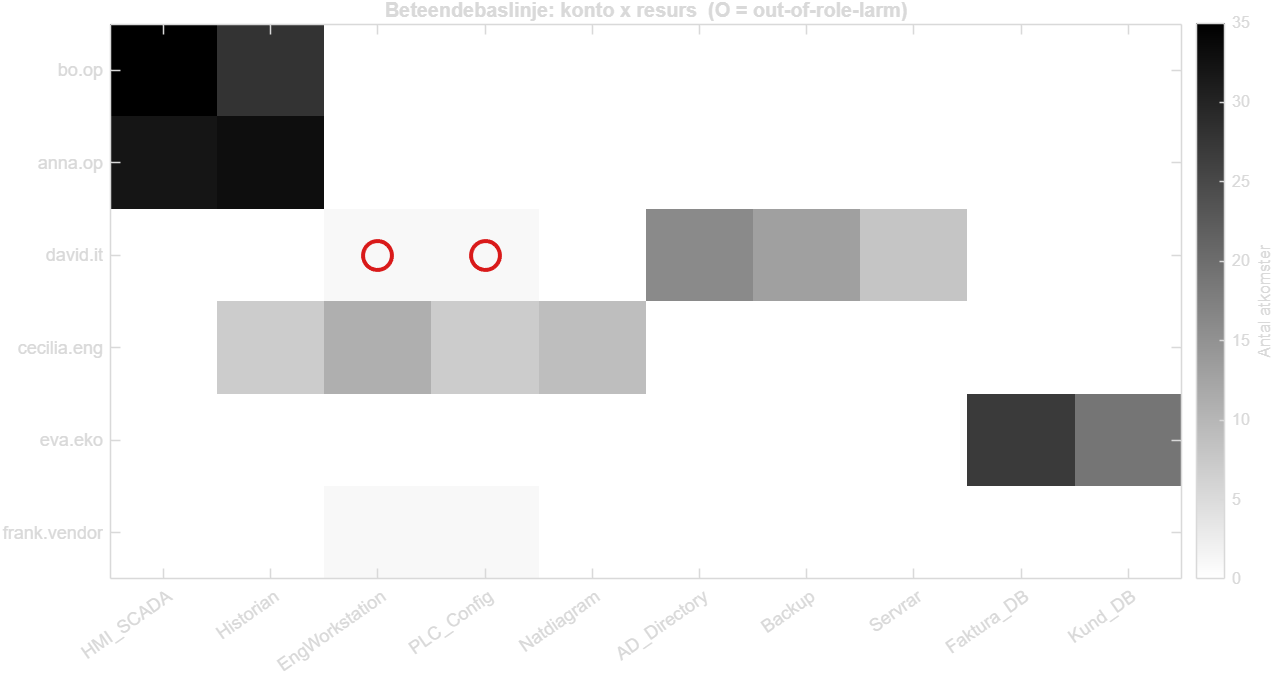
\includegraphics[width=0.86\linewidth]{output/fig_access_matrix.png}\end{center}


\secbar{13. Genomförande och filer}
Jag har byggt hela systemet i MATLAB och Simulink. Jag simulerade fjärrvärmedriften
(framlednings- och returtemperatur, flöde, pump och tryck) utifrån utomhustemperatur och
värmebehov, och injicerade fyra angreppsscenarier med känt facit. Jag tränade en normalprofil på en
ren baslinjeperiod och byggde en detektor som larmar på multivariata avvikelser (Mahalanobis-avstånd),
brutna fysikaliska samband (givarförfalskning) och förlorad telemetri. Jag modellerade även ett
hotscenario från phishing till ransomware, kopplat till MITRE ATT\&CK for ICS, med simulerade
IT-indikatorer. Rapporterna genereras automatiskt ur koden: \texttt{runDemo} kör hela kedjan
(simulera $\rightarrow$ injicera $\rightarrow$ detektera $\rightarrow$ figurer + rapport) och
\texttt{ot\_threat} skapar hotrapporten. En Simulink-modell (\texttt{ot\_security\_demo}) visar samma
detektion som ett strömmande dataflöde med funktionsblock, och \texttt{ot\_live} spelar upp förloppet
live med larm och händelselogg. Ett kompletterande UEBA-lager (\texttt{ot\_ueba}) bevakar konfidentialitet genom att lära in varje kontos normala beteende och larma på obehörig åtkomst till annars normala data.

\begin{tabularx}{\linewidth}{@{}l X@{}}
\rowcolor{th}\color{white}\textbf{Fil} & \color{white}\textbf{Funktion}\\
runDemo.m & Kör hela kedjan och genererar OT-rapport + hotrapport\\
ot\_simulate.m & Simulerar fjärrvärme-telemetri (normaldrift)\\
ot\_inject\_attacks.m & Injicerar fyra angreppsscenarier med facit\\
ot\_detect.m & Detektor: Mahalanobis + fysik-residualer + tillgänglighet\\
ot\_report.m, ot\_risk.m & Figurer, riskmodell och OT-rapport\\
ot\_killchain.m, ot\_threat.m & Kill-chain (ATT\&CK for ICS), IT-indikatorer, hotrapport\\
ot\_live.m & Live-animerad uppspelning av angrepp och detektion\\
ot\_build\_simulink.m, dh\_control\_loop.slx & Reglerloop (PI-regulator + värmeväxlare)\\
ot\_build\_demo.m, ot\_security\_demo.slx & Strömmande Simulink-demo med funktionsblock\\
OTSecurityMonitor.m & Interaktiv dashboard-app\\
runAccessDemo.m & Kör UEBA-kedjan (konfidentialitet) och genererar figurer\\
ot\_access\_sim.m, ot\_access\_inject.m & Simulerar åtkomstloggar och injicerar fyra konfidentialitetshot\\
ot\_ueba.m, ot\_access\_report.m & Beteendebaslinje + UEBA-score, klassning och figurer\\
\end{tabularx}

\vspace{6pt}{\color{gray}\small\textit{Obs: syntetisk data för demonstration. Modellen är förenklad
och visar metodik och arbetssätt, inte faktiska värden från någon specifik organisation. Byggd i
MATLAB/Simulink med stöd av MATLAB Agentic Toolkit.}}


\newpage
\secbar{Bilaga A. Auto-ifylld anmälan (exempel: INC-2026-004)}
{\color{gray}\small Genererad automatiskt av \texttt{ot\_autoreport} vid detektion. Förenklad mall för demonstration --- ersätter inte officiella anmälningsformulär.}

\newcommand{\fld}[2]{\textbf{#1:} & #2\\}
\renewcommand{\arraystretch}{1.2}

{\color{th}\textbf{1. NIS2 / cybersäkerhetslagen --- tidig varning (24h) och anmälan (72h)}}\par
\begin{tabularx}{\linewidth}{@{}p{4.6cm} X@{}}
\fld{Verksamhet}{Energibolag AB (exempel) --- Energi (fjärrvärme)}
\fld{Kontakt}{Informationssäkerhetssamordnare}
\fld{Incident-ID}{INC-2026-004}
\fld{Upptäckt}{2026-01-18 03:05}
\fld{Typ}{Ransomware-lik OT-störning (tillgänglighetsstörning)}
\fld{CSF-funktion}{RC.RP / DE.CM \quad Allvar: 5/5}
\fld{Preliminär bedömning}{Misstänkt angrepp mot OT/styrsystem; påverkan på övervakning och leverans utreds.}
\fld{Gränsöverskridande påverkan}{Nej (bedöms preliminärt)}
\fld{Tidig varning (24h)}{2026-01-19 03:05}
\fld{Incidentanmälan (72h)}{2026-01-21 03:05}
\fld{Slutrapport (1 månad)}{2026-02-18 03:05}
\fld{Mottagare}{MSB}
\end{tabularx}

\vspace{6pt}{\color{th}\textbf{2. GDPR --- personuppgiftsincident (Art.\,33, anmälan inom 72h)}}\par
\begin{tabularx}{\linewidth}{@{}p{4.6cm} X@{}}
\fld{Dataskyddsombud}{Dataskyddsombud (DPO)}
\fld{Kategorier av uppgifter}{Kunduppgifter (faktura/mätvärden) --- omfattning utreds}
\fld{Uppskattat antal registrerade}{Utreds}
\fld{Sannolika konsekvenser}{Risk för konfidentialitetsförlust vid dataexfiltrering}
\fld{Åtgärder}{Inneslutning, återställning från backup, förstärkt övervakning}
\fld{Anmälan till IMY (72h)}{2026-01-21 03:05}
\end{tabularx}

\vspace{6pt}{\color{th}\textbf{3. Säkerhetsskydd --- skyndsam anmälan}}\par
\begin{tabularx}{\linewidth}{@{}p{4.6cm} X@{}}
\fld{Bedömning}{Händelsen kan ha betydelse för säkerhetskänslig verksamhet}
\fld{Åtgärd}{Skyndsam anmälan till tillsynsmyndighet / Säkerhetspolisen}
\end{tabularx}


\end{document}
